\chapter{Getting started with Dresden OCL2 for Eclipse}
\label{chapter:introduction}

\begin{flushright}
\textit{Chapter written by Claas Wilke}
\end{flushright}

This Chapter generally introduces into \keyword{\acl{DOT4Eclipse}}. \acl{DOT4Eclipse} is the last version of the \keyword{\acl{DOT}} and is based on a \keyword{Pivot Model}. The pivot model was developed by Matthias Br�uer and is described in his Gro�er Beleg (Minor Thesis) \cite{GB:Braeuer}. Further information about the toolkit is available at the website of the \acl{DOT} \cite{WWW:toolkit}. This Chapter starts with the installation of the needed \keyword{Eclipse} plug-ins to run \acl{DOT4Eclipse}. Afterwards, it describes how to load a domain-specific model, an instance of such a model, and \acs{OCL} constraints defined on such a model.
  


\section{How to Install Dresden OCL2 for Eclipse}
	
Four different possibilities exist to install \acl{DOT4Eclipse}. (1) You may install the plug-ins using the update site available at \cite{WWW:toolkitUpdatesite}, (2) you may install the plug-ins using the binary distribution available at the SourceForge project site \cite{WWW:toolkitSourceforge}, (3) you may run the the source code distribution available at the SourceForge project site \cite{WWW:toolkitSourceforge}, or (4) you may checkout and run the source code distribution from the \acs{SVN} available at \cite{WWW:toolkitSVN}. This Section will explain the possibilities (1) and (4).
	
	
\subsection{Installing Dresden OCL2 for Eclipse using the Eclipse Update Site}
	
To install \acl{DOT4Eclipse} via the \keyword{Eclipse Update Site}, you have to start an \keyword{Eclipse} instance and select the menu option \eclipse{Help -> Install New Software ...}. Enter the path

\url{http://dresden-ocl.svn.sourceforge.net/svnroot/dresden-ocl/trunk/ocl20forEclipse/updatesite/tudresden.ocl20.updatesite\_1.2.0}

and press the \eclipse{Add...} button (see Figure \ref{pic:intro:updateSite01}). In the new opened window you can additionaly enter a name for the update site (see Figure \ref{pic:intro:updateSite02}).

\begin{figure}[!htbp]
	\centering
	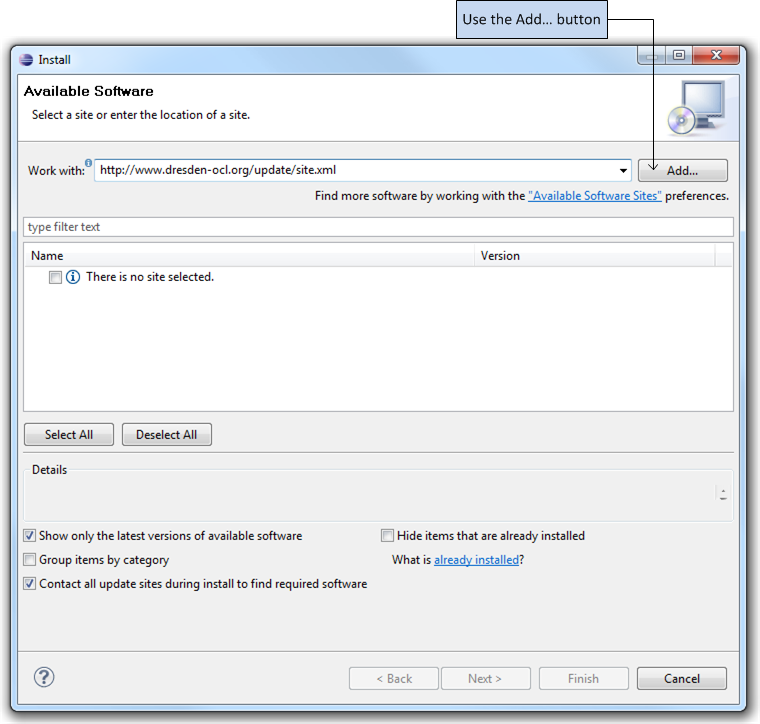
\includegraphics[width=1.0\linewidth]{figures/introduction/updateSite01}
	\caption{Adding an Eclipse Update Site (Step 1).}
	\label{pic:intro:updateSite01}
\end{figure}

\begin{figure}[!htbp]
	\centering
	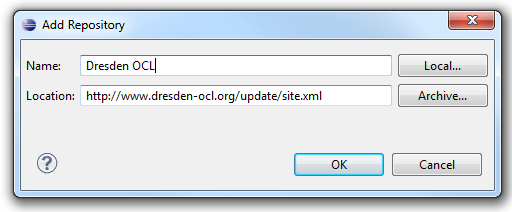
\includegraphics[width=0.6\linewidth]{figures/introduction/updateSite02}
	\caption{Adding an Eclipse Update Site (Step 2).}
	\label{pic:intro:updateSite02}
\end{figure}

Now you can select the features of \acl{DOT4Eclipse} which you want to install. Select them and click on the \eclipse{Next >} button (see figure \ref{pic:intro:updateSite03}). An overview about all features of \acl{DOT4Eclipse} can be found in table \ref{tab:plugins}. Follow the wizard and agree with the user license. Then the Toolkit will be installed. Afterwards, you should restart your Eclipse application to finish the installation.

\begin{figure}[t]
	\centering
	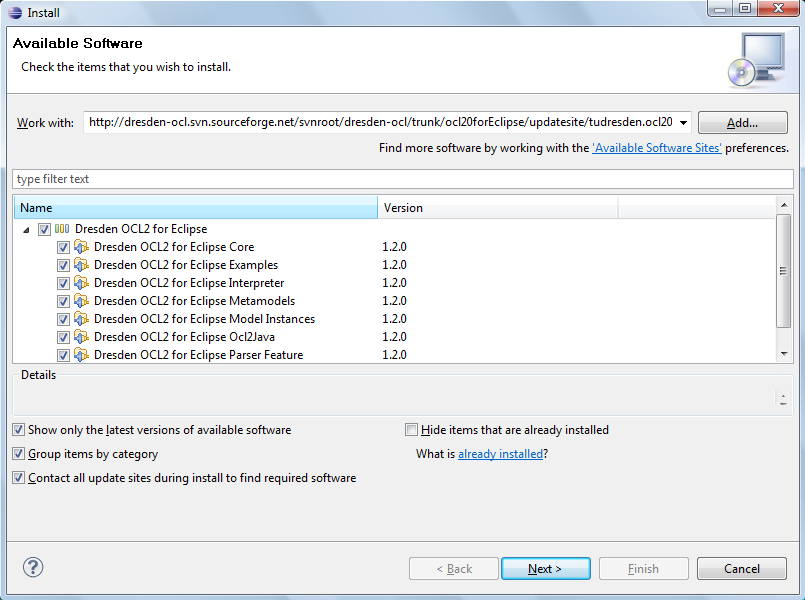
\includegraphics[width=1.0\linewidth]{figures/introduction/updateSite03}
	\caption{Selecting features of Dresden OCL2 for Eclipse.}
	\label{pic:intro:updateSite03}
\end{figure}
	
	
	
\subsection{Importing Dresden OCL2 for Eclipse from the SVN}

To use \acl{DOT4Eclipse} by checking out the source code from the \acs{SVN} you need to install a \acs{SVN} client. In the following the use the \keyword{Eclipse Subversive} plug-in and at least one of the \keyword{\acs{SVN} Connectors} available at \cite{WWW:eclipseSubversive}.

After installing Eclipse Subversive, a new \keyword{Eclispe Perspective} for access to \acs{SVN} should exist. The perspective can be opened via the menu \eclipse{Window > Open Perpective > Other... > SVN Repository Exploring}. In the view \eclipse{\acs{SVN} Repositories} you can add a new repository (see Figure \ref{pic:intro:svn01}) using the URL \url{https://dresden-ocl.svn.sourceforge.net/svnroot/dresden-ocl/}.

\begin{figure}[!htbp]
	\centering
	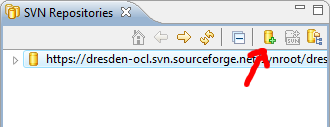
\includegraphics[width=0.5\linewidth]{figures/introduction/svn01}
	\caption{Adding a SVN repository.}
	\label{pic:intro:svn01}
\end{figure}

After pressing the \eclipse{Finish} button the \acs{SVN} repository root should the visible in the \eclipse{\acs{SVN} Repositories} view. To checkout the plug-ins, you now select them in the repository directory \reference{trunk/ocl20forEclipse/eclipse} and use the \eclipse{Checkout...} function in the context menu (see figure \ref{pic:intro:svn02}).
	
	
\begin{figure}[!htbp]
	\centering
	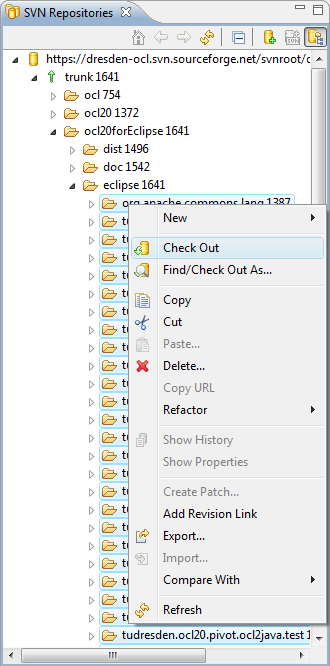
\includegraphics[width=0.5\linewidth]{figures/introduction/svn02}
	\caption{Checkout of the Dresden OCL2 Toolkit plug-in projects.}
	\label{pic:intro:svn02}
\end{figure}


\subsection{Which Plug-ins do I need at least?}

An often asked question is ``Which plug-ins are at least required to run \acl{DOT4Eclipse}?'' Well, the answer is: ``That depends.''

That depends on the things you want to do with \acl{DOT4Eclipse}. Table \ref{tab:plugins} shows a list of the current plug-ins of \acl{DOT4Eclipse}, that are related to different features. You should install at least the \keyword{Core} feature, at least one of the \keyword{Metamodels}, and the \keyword{Parser} feature. The \keyword{Interpreter} and \keyword{OCL2Java} features are only required if you want to interpret constraints or to generate code from constraints. If you import or interpret model instances, you need to install the \keyword{Model Instances} feature as well. The examples of the \keyword{Example} feature are only required to run the examples provided in the tutorials available at \cite{WWW:toolkit}. We recommend to install all provided features.
		


\subsection{Building the OCL2 Parser}
	
If you decided to run \acl{DOT4Eclipse} as source code plug-ins from an Eclipse workspace, you need to build the \keyword{OCL2 Parser} via an \keyword{Ant} build script. If you installed the Toolkit using the update site, you can skip this Subsection of the tutorial.
  
To build the \acs{OCL}2 Parser select the file \reference{build.xml} in the project \reference{tudresden.\linebreak[0]ocl20.pivot.ocl2parser} and open the context menu via a right mouse click. Select the function \eclipse{Run As ... > Ant Build ...} (see Figure \ref{pic:intro:parserbuild01}).

\begin{figure}[b]
	\centering
	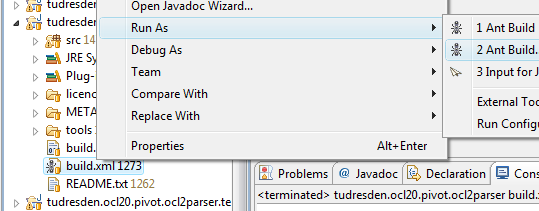
\includegraphics[width=0.8\linewidth]{figures/introduction/parserbuild01}
	\caption{Executing the OCL2 parser build script.}
	\label{pic:intro:parserbuild01}
\end{figure}
	
A new window should open. Select in the sub menu \keyword{\acs{JRE}} the check box \keyword{Run in the same \acs{JRE} as the workspace} and click on the button \keyword{OK} (see figure \ref{pic:intro:parserbuild02}). Afterwards the \acs{OCL}2 Parser should be generated without errors. If an error like ``Unable to find javac compiler.'' occurs, you might be trying to run the \keyword{Ant} script with a \keyword{\acl{JRE}} instead of a \keyword{\acs{JDK}} (For errors like) use the \eclipse{Installed JREs...} button in the same window to select a JDK instead.
	
\begin{figure}[!htbp]
	\centering
	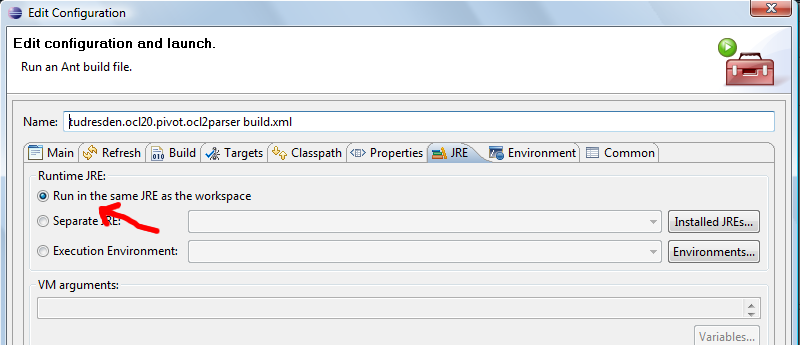
\includegraphics[width=1.0\linewidth]{figures/introduction/parserbuild02}
	\caption{Settings of the JRE for the Ant build script.}
	\label{pic:intro:parserbuild02}
\end{figure}
	
After executing the build script successfully you need to update the projects in your workspace. Update the project \reference{tudresden.ocl20.pivot.oclparser} via context menu (\eclipse{Refresh}, see figure \ref{pic:intro:parserbuild03}).

\begin{figure}[!htbp]
	\centering
	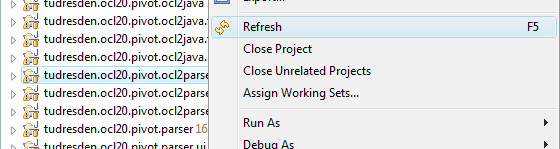
\includegraphics[width=0.8\linewidth]{figures/introduction/parserbuild03}
	\caption{Refreshing the project ``tudresden.ocl20.pivot.oclparser''.}
	\label{pic:intro:parserbuild03}
\end{figure}
	
Additionally you need to recompile all depending projects. Select the function \eclipse{Project > Clean... > Clean all projects} in the Eclipse menu to clean all projects. Now all the projects should not contain any errors anymore and should be executable.



\section{Loading Models, Model Instances and OCL Constraints}

If you installed the \acl{DOT4Eclipse} using the update site, you can execute the toolkit by re-starting your Eclipse distribution. If you imported the Toolkit as source code plug-ins into an Eclipse workspace, you have to start a new Eclipse instance. You can start a new instance via the menu \eclipse{Run > Run As > Eclipse Application}. If the menu \eclipse{Eclipse Application} is not available or disabled you need to select one of the plug-ins of the toolkit first.



\subsection{The Simple Example}
\label{intro:simpleExample}

The use of \acl{DOT4Eclipse} is explained using the \keyword{Simple Example} which is located in the plug-in package \reference{tudresden.ocl20.pivot.examples.\linebreak[0]simple}. Figure \ref{pic:examples:simple01} shows the class diagram of the Simple Example.

\begin{figure}[!htbp]
	\centering
	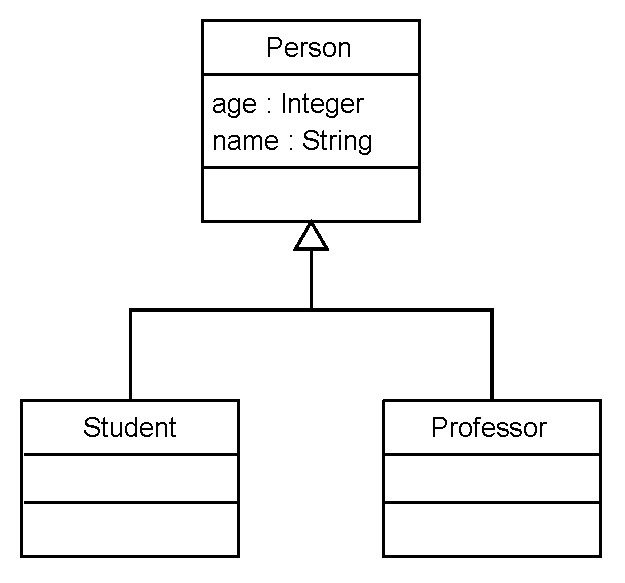
\includegraphics[width=0.5\linewidth]{figures/examples/simple01}
	\caption{The class diagram described by the simple example model.}
	\label{pic:examples:simple01}
\end{figure}

\acl{DOT4Eclipse} provides more examples than the \keyword{Simple Example}. The different examples use different meta-models which is possible with the \textit{Pivot Model} architecture of the Toolkit. An overview about all examples provided with \keyword{Dresden OCL2 for Eclipse} is listed in table \ref{tab:examples}. The Simple Example can be used with two different meta-models. These are \keyword{\acs{UML} 2.0} (based on \keyword{\acs{Eclipse MDT} \acs{UML}2}) and \keyword{\acs{EMF} Ecore}.
	

\subsection{Loading a Domain-Specific Model}
	
After starting Eclipse you have to load a model into the toolkit. If the plug-ins of \acl{DOT4Eclipse} have been installed using the update site, the Simple Example plug-in have to be imported into the \keyword{Workspace} first. Create a new Java project into your workspace and select the \keyword{Import Wizard} \eclipse{General > Archive File}. In the following window select the \eclipse{plugins} directory in your Eclipse root folder, select the archive \reference{tudresden.ocl20.pivot.examples.\linebreak[0]simple\_1.0.0.jar} and click the \eclipse{Finish} button.

Now you can load a model. Select the menu option \eclipse{Dresden OCL2 > Load Model}. In the opened wizard you have to select a model file and a meta-model for the model (see Figure \ref{pic:intro:loadmodel01}). Click the button \eclipse{Browse Workspace...} and select the file \reference{model/simple.uml} inside the Simple Example Project. Then select the meta-model \acs{UML}2 and press the button \eclipse{Finish}.

\begin{figure}[!htbp]
	\centering
	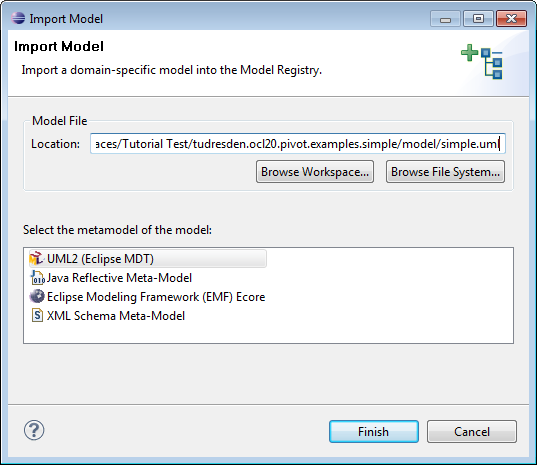
\includegraphics[width=0.8\linewidth]{figures/introduction/loadmodel01}
	\caption{Loading a domain specific model.}
	\label{pic:intro:loadmodel01}
\end{figure}
	
Figure \ref{pic:intro:loadmodel02} shows the loaded Simple Example model, which uses \acs{UML}2 as its meta-model. Via the menu button of the \eclipse{Model Browser} (the little triangle in the right top corner) you can switch between different models (see Figure \ref{pic:intro:loadmodel03}).
	
\begin{figure}[!htbp]
	\centering
	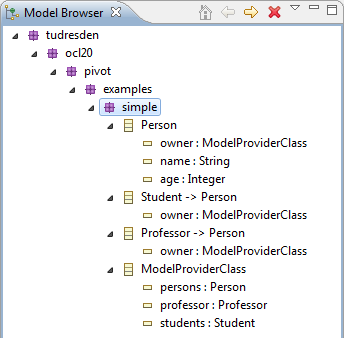
\includegraphics[width=0.5\linewidth]{figures/introduction/loadmodel02}
	\caption{The loaded Simple Example model in the model browser.}
	\label{pic:intro:loadmodel02}
\end{figure}

\begin{figure}[!htbp]
	\centering
	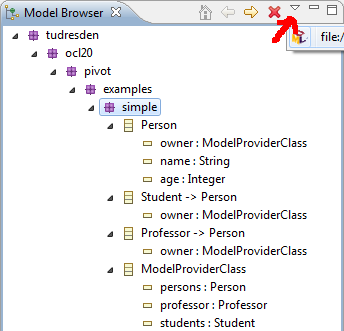
\includegraphics[width=0.6\linewidth]{figures/introduction/loadmodel03}
	\caption{You can switch between different models using the little triangle.}
	\label{pic:intro:loadmodel03}
\end{figure}

	
\subsection{Loading a Model Instance}
\label{intro:loadModel}
	
After loading a model, you can load a \keyword{model instance} using another wizard. Use the menu option \eclipse{Dresden OCL2 > Load Model Instance}. In the opened wizard you have to select a model instance (in this tutorial we used the file \reference{bin/tudresden/ocl20/\linebreak[0]pivot/examples/ModelProviderClass.class} of the Simple Example (see Figure \ref{pic:intro:loadInstance01}). Besides the model instance resource you have to select a model for which the model instance shall be loaded and the type of model instance you want to load (we want to load a \keyword{Java Instance}).

\begin{figure}[!htbp]
	\centering
	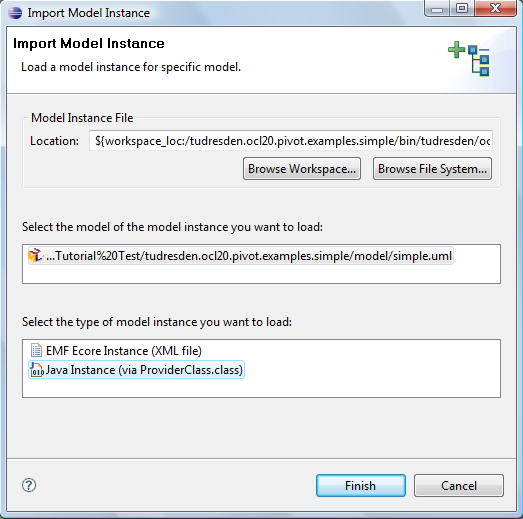
\includegraphics[width=0.8\linewidth]{figures/introduction/loadinstance01}
	\caption{Loading a simple model instance.}
	\label{pic:intro:loadInstance01}
\end{figure}
	
Figure \ref{pic:intro:loadInstance02} shows the loaded model instance of the Simple Example model. Like in the model browser you can switch between different model instances. Note that the model instance browser only shows the model instances of the model actually selected in the model browser. By switching the domain specific model, you also switch the pool of model instances available in the model instance browser.

\begin{figure}[!htbp]
	\centering
	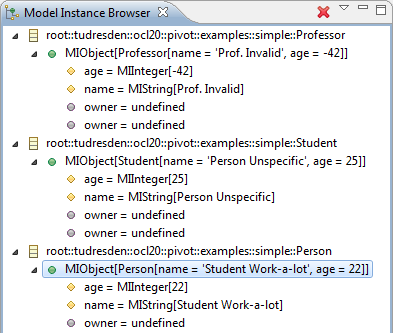
\includegraphics[width=0.5\linewidth]{figures/introduction/loadinstance02}
	\caption{A simple model instance in the Model Instance Browser.}
	\label{pic:intro:loadInstance02}
\end{figure}

	

\subsection{Parsing OCL expressions}
	
Before you can work with \acs{OCL} constraints you have to load them like the domain-specific model and the model instance into the toolkit. Use the menu option \eclipse{Dresden OCL2 > OCL Expressions} and select an \acs{OCL} file. In this tutorial we used the \acs{OCL} file \reference{constraints/invariants.ocl} of the Simple Example. (see Figure \ref{pic:intro:loadconstraints01}). The constraints of the file \reference{constraints/invariants.ocl} are shown in listing \ref{list:intro:constraints01}.

The expressions of the selected \acs{OCL} file are loaded into the actually selected model. Figure \ref{pic:intro:loadconstraints01} shows the \reference{Model Browser} containing the model and the parsed expressions.

\begin{figure}[b]	
\lstset{
  language=OCL
}
\begin{lstlisting}[caption={The invariants of the simple examples.}, captionpos=b, label=list:intro:constraints01]
package tudresden::ocl20::pivot::examples::simple

-- The age of Person can't be negative.
context Person
inv: age >= 0

-- Students should be 16 or older.
context Student
inv: age > 16

-- Proffesors should be at least 30.
context Professor
inv: not (age < 30)

endpackage
\end{lstlisting}
\end{figure}

\begin{figure}[p]
	\centering
	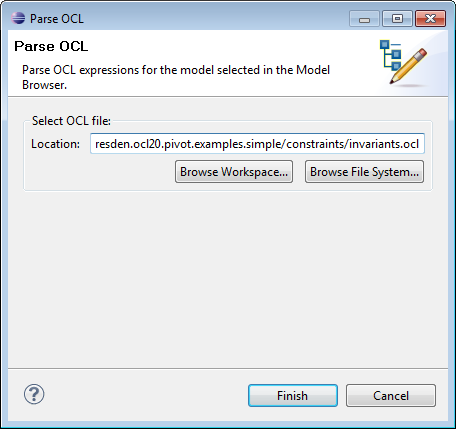
\includegraphics[width=0.8\linewidth]{figures/introduction/loadconstraints01}
	\caption{The import of OCL expressions.}
	\label{pic:intro:loadconstraints01}
	
	\centering
	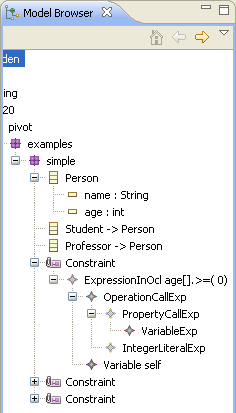
\includegraphics[width=0.5\linewidth]{figures/introduction/loadconstraints02}
	\caption{Parsed expressions and the model in the Model Browser.}
	\label{pic:intro:loadconstraints02}
\end{figure}
	
	
\section{Summary}
  
This Chapter described how to use \acl{DOT4Eclipse}. It explained how to install the toolkit's plug-ins. Afterwards, the loading of domain-specific models, model instances and \acs{OCL} constraints into the toolkit has been explained.

Now, the imported models can be used to use the tools provided with \acl{DOT4Eclipse}. For example you can use the \keyword{OCL2 Interpreter} of \acl{DOT4Eclipse} to interpret \acs{OCL} constraints for a given model and model instance (as explained in Chapter \ref{chapter:interpretation}) or you can use the \keyword{OCL22Java Code Generator} to generate \keyword{AspectJ} code for a loaded model and \acs{OCL} constraints (as explained in Chapter \ref{chapter:codeGeneration}).